\documentclass[a4paper]{article}
\usepackage{geometry}
\usepackage{graphicx}
\usepackage{natbib}
\usepackage{amsmath}
\usepackage{amssymb}
\usepackage{amsthm}
\usepackage{paralist}
\usepackage{epstopdf}
\usepackage{tabularx}
\usepackage{longtable}
\usepackage{multirow}
\usepackage{multicol}
\usepackage[hidelinks]{hyperref}
\usepackage{fancyvrb}
\usepackage{algorithm}
\usepackage{algorithmic}
\usepackage{float}
\usepackage{paralist}
\usepackage[svgname]{xcolor}
\usepackage{enumerate}
\usepackage{array}
\usepackage{times}
\usepackage{url}
\usepackage{fancyhdr}
\usepackage{comment}
\usepackage{environ}
\usepackage{times}
\usepackage{textcomp}
\usepackage{caption}
\usepackage{color}
\usepackage{xcolor}
\usepackage{listings}
\usepackage{caption}
\usepackage{subcaption}

\urlstyle{rm}

\setlength\parindent{0pt} % Removes all indentation from paragraphs
\theoremstyle{definition}
\newtheorem{definition}{Definition}[]
\newtheorem{conjecture}{Conjecture}[]
\newtheorem{example}{Example}[]
\newtheorem{theorem}{Theorem}[]
\newtheorem{lemma}{Lemma}
\newtheorem{proposition}{Proposition}
\newtheorem{corollary}{Corollary}

\floatname{algorithm}{Procedure}
\renewcommand{\algorithmicrequire}{\textbf{Input:}}
\renewcommand{\algorithmicensure}{\textbf{Output:}}
\newcommand{\abs}[1]{\lvert#1\rvert}
\newcommand{\norm}[1]{\lVert#1\rVert}
\newcommand{\RR}{\mathbb{R}}
\newcommand{\CC}{\mathbb{C}}
\newcommand{\Nat}{\mathbb{N}}
\newcommand{\br}[1]{\{#1\}}
\DeclareMathOperator*{\argmin}{arg\,min}
\DeclareMathOperator*{\argmax}{arg\,max}
\renewcommand{\qedsymbol}{$\blacksquare$}

\definecolor{dkgreen}{rgb}{0,0.6,0}
\definecolor{gray}{rgb}{0.5,0.5,0.5}
\definecolor{mauve}{rgb}{0.58,0,0.82}

\newcommand{\Var}{\mathrm{Var}}
\newcommand{\Cov}{\mathrm{Cov}}

\newcommand{\vc}[1]{\boldsymbol{#1}}
\newcommand{\xv}{\vc{x}}
\newcommand{\Sigmav}{\vc{\Sigma}}
\newcommand{\alphav}{\vc{\alpha}}
\newcommand{\muv}{\vc{\mu}}

\newcommand{\red}[1]{\textcolor{red}{#1}}

\def\x{\mathbf x}
\def\y{\mathbf y}
\def\w{\mathbf w}
\def\v{\mathbf v}
\def\E{\mathbb E}
\def\V{\mathbb V}

% TO SHOW SOLUTIONS, include following (else comment out):
\newenvironment{soln}{
    \leavevmode\color{blue}\ignorespaces
}{}


\hypersetup{
%    colorlinks,
    linkcolor={red!50!black},
    citecolor={blue!50!black},
    urlcolor={blue!80!black}
}

\geometry{
  top=1in,            % <-- you want to adjust this
  inner=1in,
  outer=1in,
  bottom=1in,
  headheight=3em,       % <-- and this
  headsep=2em,          % <-- and this
  footskip=3em,
}


\pagestyle{fancyplain}
\lhead{\fancyplain{}{Homework 2}}
\rhead{\fancyplain{}{CS 760 Machine Learning}}
\cfoot{\thepage}

\title{\textsc{Homework 2}} % Title

%%% NOTE:  Replace 'NAME HERE' etc., and delete any "\red{}" wrappers (so it won't show up as red)

\author{
\red{$>>$Anudeep Kumar$<<$} \\
\red{$>>$9084607069$<<$}\\
} 

\date{}

\begin{document}

\maketitle 


\textbf{Instructions:} 
Use this latex file as a template to develop your homework. Submit your homework on time as a single pdf file to Canvas. Please wrap your code and upload to a public GitHub repo, then attach the link below the instructions so that we can access it. You can choose any programming language (i.e. python, R, or MATLAB), as long as you implement the algorithm from scratch (e.g. do not use sklearn on questions 1 to 7 in section 2). Please check Piazza for updates about the homework.

\section{A Simplified Decision Tree}
You are to implement a decision-tree learner for classification.
To simplify your work, this will not be a general purpose decision tree.  Instead, your program can assume that
\begin{itemize}
\item each item has two continuous features $\x \in \RR^2$
\item the class label is binary and encoded as $y \in \{0,1\}$
\item data files are in plaintext with one labeled item per line, separated by whitespace:
$$x_{11} \quad x_{12} \quad y_1$$
$$...$$
$$x_{n1} \quad x_{n2} \quad y_n$$
\end{itemize}

Your program should implement a decision tree learner according to the following guidelines:
\begin{itemize}
\item Candidate splits $(j,c)$ for numeric features should use a threshold $c$ in feature dimension $j$ in the form of $x_{\cdot j}\ge c$.
\item $c$ should be on values of that dimension present in the training data; i.e. the threshold is on training points, not in between training points. You may enumerate all features, and for each feature, use all possible values for that dimension.
\item You may skip those candidate splits with zero split information (i.e. the entropy of the split), and continue the enumeration.
\item The left branch of such a split is the ``then'' branch, and the right branch is ``else''.
\item Splits should be chosen using information gain ratio. If there is a tie you may break it arbitrarily.
\item The stopping criteria (for making a node into a leaf) are that 
	\begin{itemize}
	\item the node is empty, or
	\item all splits have zero gain ratio (if the entropy of the split is non-zero), or
	\item the entropy of any candidates split is zero
	\end{itemize}
\item To simplify, whenever there is no majority class in a leaf, let it predict $y=1$.
\end{itemize}

\section{Questions}
\begin{enumerate}
\item (Our algorithm stops at pure labels) [10 pts] If a node is not empty but contains training items with the same label, why is it guaranteed to become a leaf?  Explain. You may assume that the feature values of these items are not all the same. \\
\begin{soln}
    As per the information given if at any given node the training items have same label then we can say that the probability of new label will be $~0$. In that case the Entropy $H(X)=E[log(1/P(X=x)]$\\
    Which can be expanded as :\\
    $-P(X=new)log(P(X=new)-P(X=known)logP(X=known)$\\
    $-0.0001log(1/0.0001)-0.99999log(1/0.9999)$\\
    $-0.0001*13.2-0.99999*0.000001$\\
    $~0$ \\
    Similarly for any given label the $H(S|X)$ will come out to be 0 hence 0 Information gained so we can stop at the point when value of labels are same.
\end{soln}

\item (Our algorithm is greedy)  [10 pts] Handcraft a small training set where both classes are present but the algorithm refuses to split; instead it makes the root a leaf and stop;
Importantly, if we were to manually force a split, the algorithm will happily continue splitting the data set further and produce a deeper tree with zero training error.
You should (1) plot your training set, (2) explain why.  Hint: you don't need more than a handful of items. \\
\begin{soln}
Let us consider the data as below
\begin{figure}[H]
            \centering
            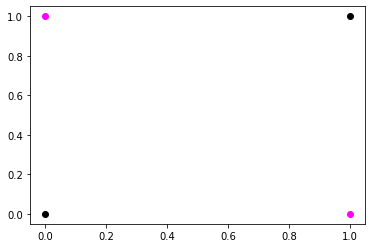
\includegraphics[scale=0.5]{XOR.png}
            \label{fig:q2}
        \end{figure}
\begin{tabular}{|c|c|c|}
            \hline
            x & y & label \\
            \hline
            0 & 0 & 0 \\
            0 & 1 & 1 \\
            1 & 0 & 1 \\
            1 & 1 & 0 \\
            \hline
        \end{tabular}
\\The total entropy is :\\
$H(label)=-1/2log(2)-1/2log(2)=-log(2)=-1$\\
Now to define the node we calculate the Information gained for y = 1 and y = 0 , which comes out to be :\\
$IG(label|y)=H(label)-P(y=0)H(y=0)-P(y=1)H(y=1)$\\
$IG(label|y)=-1-1/2(-1/2log(2)-1/2log(2))-1/2(-1/2log(2)-1/2(log2))=-1+1=0$\\
Similarly for $IG(label|x)$ the Information gained is 0. So the decision tree wont split. It will make the root a leaf and stop.\\
\\ We can observe that if we explicitly force a split such as:\\
Node1: X==1 ? (True:Node2 ;  False:Node3)\\
Node2: Y==1 ? (True:Class0; False:Class1)\\
Node3: Y==0 ? (True:Class0; False:Class1)\\
Hence we can make the tree split explicitly and Information gain being zero cannot be the only stopping criteria.

    
\end{soln}

\item (Information gain ratio exercise)  [10 pts] Use the training set Druns.txt.  For the root node, list all candidate cuts and their information gain ratio. If the entropy of the candidate split is zero, please list its mutual information (i.e. information gain). Hint: to get $\log_2(x)$ when your programming language may be using a different base, use \verb|log(x)/log(2)|. Also, please follow the split rule in the first section. \\
\begin{soln}
    We start with finding out the entropy of Y which can take the value 0 or 1,in our data set. Then for each columns, we find the Information gains if we made split at that point. For the first column we had 0.1 and 0. We calculated the entropy for x being greater than equal or less than 0.1 and 0 and corresponding number of labels being 0 or 1. We calculate corresponding probabilities and find the Entropy which is listed as below:\\
    \begin{tabular}{|c|c|c|c|}
        \hline
        \textbf{Feature} & \textbf{Cutoff} & \textbf{Info. Gain Ratio} & \textbf{Info. Gain} \\
        \hline
        \textit{X1} & \textit{0.0} & -- & \textit{0.0} \\
        X1 & 0.1 & 0.10051807676021828 & 0.04417739186726133 \\
        \hline
        \textit{X2} & \textit{-2.0} & -- & \textit{0.0} \\
        X2 & -1.0 & 0.10051807676021828 & 0.04417739186726133 \\
        X2 & 0.0 & 0.05595375963126383 & 0.03827452220629246\\
        X2 & 1.0 & 0.005780042205152189 & 0.004886164091842726 \\
        X2 & 2.0 & 0.001144349517276632 & 0.0010821659130775263 \\
        X2 & 3.0 & 0.016411136842102023 & 0.016313165825732057 \\
        X2 & 4.0 & 0.049749064181778435 & 0.04945207278939401 \\
        X2 & 5.0 & 0.11124029586339801 & 0.10519553207004628 \\
        X2 & 6.0 & 0.236099606143608 & 0.19958702318968735 \\
        X2 & 7.0 & 0.05595375963126383 & 0.03827452220629246 \\
        X2 & 8.0 & 0.4301569161309807 & 0.18905266854301617 \\
        \hline
    \end{tabular}
\end{soln}

\item (The king of interpretability)  [10 pts] Decision tree is not the most accurate classifier in general.  However, it persists.  This is largely due to its rumored interpretability: a data scientist can easily explain a tree to a non-data scientist.  Build a tree from D3leaves.txt.  Then manually convert your tree to a set of logic rules.  Show the tree\footnote{When we say show the tree, we mean either the standard computer science tree view, or some crude plaintext representation of the tree -- as long as you explain the format.  When we say visualize the tree, we mean a plot in the 2D $\x$ space that shows how the tree will classify any points.} and the rules. \\
\begin{soln}
    From the above set of rules we make a tree. The tree made by the logic is :\\

    $Node X_1>=10 : (True: Class_1, False: NodeX_2)$\\
    $Node X_2>=3  : (True: Class_1, False: Class_0)$

\end{soln}

\item (Or is it?)  [20 pts] For this question only, make sure you DO NOT VISUALIZE the data sets or plot your tree's decision boundary in the 2D $\x$ space.  If your code does that, turn it off before proceeding.  This is because you want to see your own reaction when trying to interpret a tree.  You will get points no matter what your interpretation is.
And we will ask you to visualize them in the next question anyway.
  \begin{itemize}
  
  \item Build a decision tree on D1.txt.  Show it to us in any format (e.g. could be a standard binary tree with nodes and arrows, and denote the rule at each leaf node; or as simple as plaintext output where each line represents a node with appropriate line number pointers to child nodes; whatever is convenient for you). Again, do not visualize the data set or the tree in the $\x$ input space.  In real tasks you will not be able to visualize the whole high dimensional input space anyway, so we don't want you to ``cheat'' here.
  \\
  \begin{soln}
      $Node X_2\ge0.201829:(True : Class_1, False: Class_0) $
  \end{soln}
  
  \item Look at your tree in the above format (remember, you should not visualize the 2D dataset or your tree's decision boundary) and try to interpret the decision boundary in human understandable English. 

  \begin{soln}
      From the above node representation we can observe that X2 if greater than or equal to 0.201829 the class assigned is 1 else Class is 0
  \end{soln}
  
  \item Build a decision tree on D2.txt.  Show it to us. 
  \begin{soln}
      \begin{lstlisting}
      {
  "X1": {
    ">=0.533076 then": {
      "X2": {
        ">=0.228007 then": {
          "X2": {
            ">=0.424906 then": 1,
            "else <0.424906": {
              "X1": {
                ">=0.708127 then": 1,
                "else <0.708127": {
                  "X2": {
                    ">=0.32625 then": {
                      "X1": {
                        ">=0.595471 then": {
                          "X1": {
                            ">=0.646007 then": 1,
                            "else <0.646007": {
                              "X2": {
                                ">=0.403494 then": 1,
                                "else <0.403494": 0
                              }
                            }
                          }
                        },
                        "else <0.595471": 0
                      }
                    },
                    "else <0.32625": 0
                  }
                }
              }
            }
          }
        },
        "else <0.228007": {
          "X1": {
            ">=0.887224 then": {
              "X2": {
                ">=0.037708 then": {
                  "X2": {
                    ">=0.082895 then": 1,
                    "else <0.082895": {
                      "X1": {
                        ">=0.960783 then": 1,
                        "else <0.960783": 0
                      }
                    }
                  }
                },
                "else <0.037708": 0
              }
            },
            "else <0.887224": {
              "X1": {
                ">=0.850316 then": {
                  "X2": {
                    ">=0.169053 then": 1,
                    "else <0.169053": 0
                  }
                },
                "else <0.850316": 0
              }
            }
          }
        }
      }
    },
    "else <0.533076": {
      "X2": {
        ">=0.88635 then": {
          "X1": {
            ">=0.041245 then": {
              "X1": {
                ">=0.104043 then": 1,
                "else <0.104043": {
                  "X1": {
                    ">=0.07642 then": 0,
                    "else <0.07642": 1
                  }
                }
              }
            },
            "else <0.041245": 0
          }
        },
        "else <0.88635": {
          "X2": {
            ">=0.691474 then": {
              "X1": {
                ">=0.254049 then": 1,
                "else <0.254049": {
                  "X1": {
                    ">=0.191915 then": {
                      "X2": {
                        ">=0.792752 then": 1,
                        "else <0.792752": 0
                      }
                    },
                    "else <0.191915": {
                      "X2": {
                        ">=0.864128 then": {
                          "X1": {
                            ">=0.144781 then": 1,
                            "else <0.144781": 0
                          }
                        },
                        "else <0.864128": 0
                      }
                    }
                  }
                }
              }
            },
            "else <0.691474": {
              "X2": {
                ">=0.534979 then": {
                  "X1": {
                    ">=0.426073 then": 1,
                    "else <0.426073": {
                      "X1": {
                        ">=0.409972 then": {
                          "X1": {
                            ">=0.417579 then": 0,
                            "else <0.417579": 1
                          }
                        },
                        "else <0.409972": {
                          "X1": {
                            ">=0.393227 then": {
                              "X1": {
                                ">=0.39583 then": 0,
                                "else <0.39583": 1
                              }
                            },
                            "else <0.393227": 0
                          }
                        }
                      }
                    }
                  }
                },
                "else <0.534979": 0
              }
            }
          }
        }
      }
    }
  }
}
      \end{lstlisting}
  \end{soln}
  
  \item Try to interpret your D2 decision tree. Is it easy or possible to do so without visualization? \\
  \begin{soln}
      As we can observe from the output of the code it is very difficult to interpret. The number of nodes is 30. It is not impossible but extremely hectic to visualise.Node starts at $X1 \ge0.533076$ and then keeps on bifurcating.
  \end{soln}
  
  \end{itemize}

\item (Hypothesis space)  [10 pts] For D1.txt and D2.txt, do the following separately:
  \begin{itemize}
  
  \item Produce a scatter plot of the data set.
  \begin{soln}
      We observe the D1 and D2 dataset below:\\
       \begin{figure}[H]
            \centering
            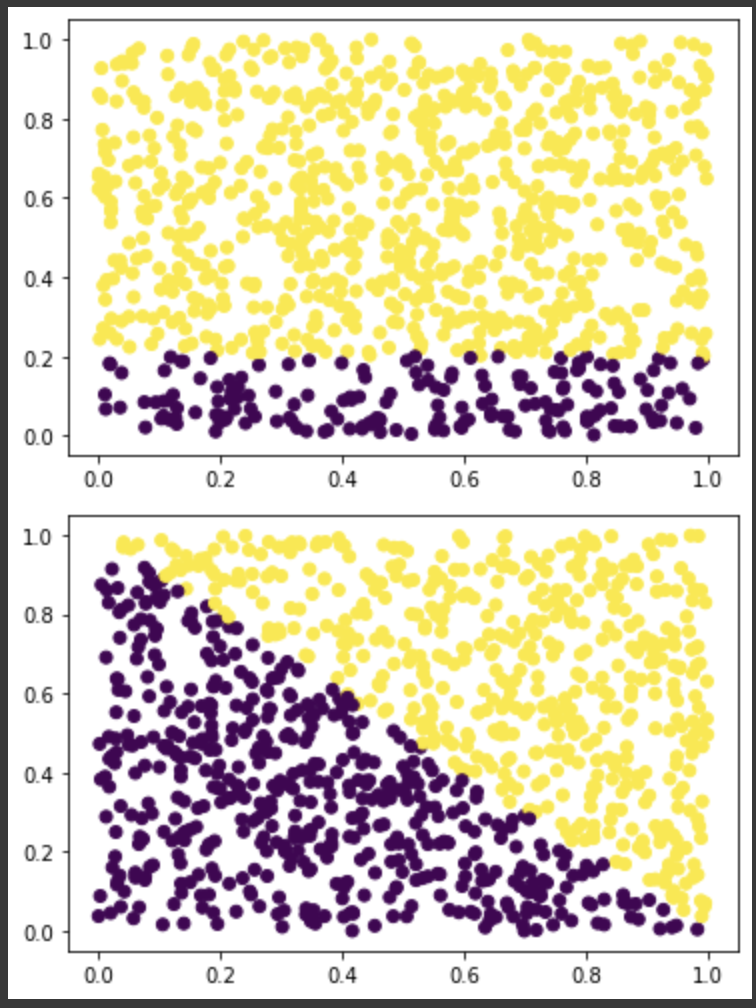
\includegraphics[scale=0.5]{datatrain.png}
            \label{fig:q2}
        \end{figure}
  \end{soln}

  \item Visualize your decision tree's decision boundary (or decision region, or some other ways to clearly visualize how your decision tree will make decisions in the feature space).
  
\begin{soln}
For this we approached with creating 10000 random variable between 0 and 1. We then pass it to the Decision Tree object and find the below prediction
    \begin{figure}[H]
            \centering
            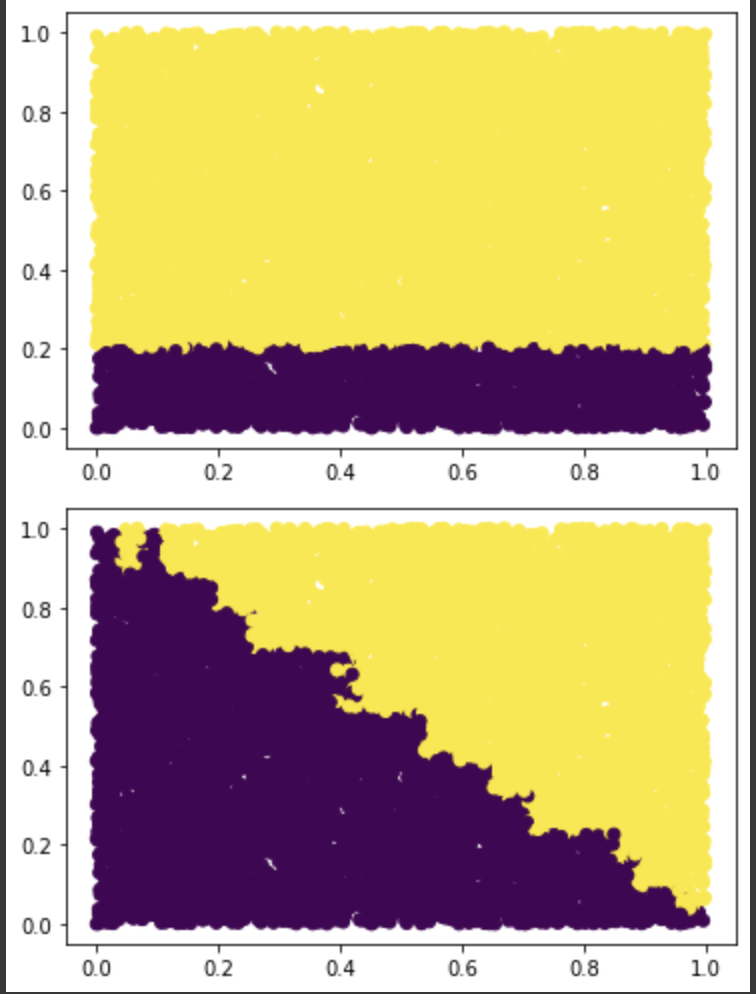
\includegraphics[scale=0.5]{datatest.png}
            \label{fig:q2}
        \end{figure}
\end{soln}
  \end{itemize}
Then discuss why the size of your decision trees on D1 and D2 differ.  Relate this to the hypothesis space of our decision tree algorithm. \\
\begin{soln}
    We saw that the decision boundary for D1 is parallel to x axis which implies x2 is independent of x1 and which was observed before earlier when 1 node was enough to decide the output.
    Similarly for D2, there were 30 nodes, and we can see that the decision boundary is somewhat following the line
    $y+x=1$.
\end{soln}

\item (Learning curve)  [20 pts] We provide a data set Dbig.txt with 10000 labeled items.  Caution: Dbig.txt is sorted.
  \begin{itemize}
  
  \item You will randomly split Dbig.txt into a candidate training set of 8192 items and a test set (the rest).  Do this by generating a random permutation, and split at 8192.
  
  \item Generate a sequence of five nested training sets $D_{32} \subset D_{128} \subset D_{512} \subset D_{2048} \subset D_{8192}$ from the candidate training set.  The subscript $n$ in $D_n$ denotes training set size.  The easiest way is to take the first $n$ items from the (same) permutation above.  This sequence simulates the real world situation where you obtain more and more training data.
  
  \item For each $D_n$ above, train a decision tree.  Measure its test set error $err_n$.  Show three things in your answer: (1) List $n$, number of nodes in that tree, $err_n$. (2) Plot $n$ vs. $err_n$.  This is known as a learning curve (a single plot). (3) Visualize your decision trees' decision boundary (five plots). \\
  \end{itemize}
  
  \begin{soln}
  \begin{center}
      
  \begin{tabular}{|c|c|}
            \hline
            Data Size & Node \\
            \hline
            32 & 6\\
            128 & 10\\
            512 & 27\\
            2048 & 64 \\
            8192 & 145 \\
            \hline
        \end{tabular}\\
  
      Data 32 Split Test Error: 16.87\%\\
      Data 128 Split Test Error: 10.9\%\\
      Data 512 Split Test Error: 5.59\%\\
      Data 2048 Split Test Error: 2.38\%\\
      Data 8192 Split Test Error: 1.27\%\\
        \end{center}
      We can observe the figure below
        \begin{figure}[H]
            \centering
            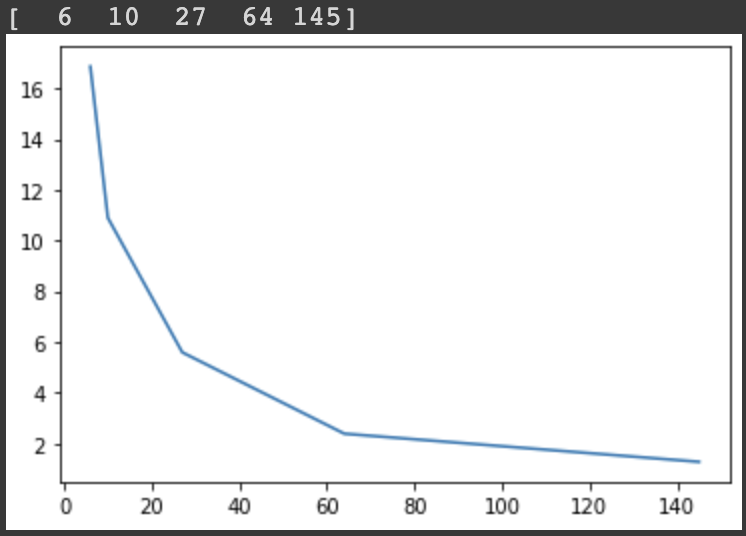
\includegraphics[scale=0.5]{error.png}
            \label{fig:q2}
            \caption{Error vs N}
        \end{figure} 
    
    The observed Training and Test plot for 5 splits are shown below:\\
    \begin{figure}[H]
        \begin{subfigure}{0.5\textwidth}
            \centering
            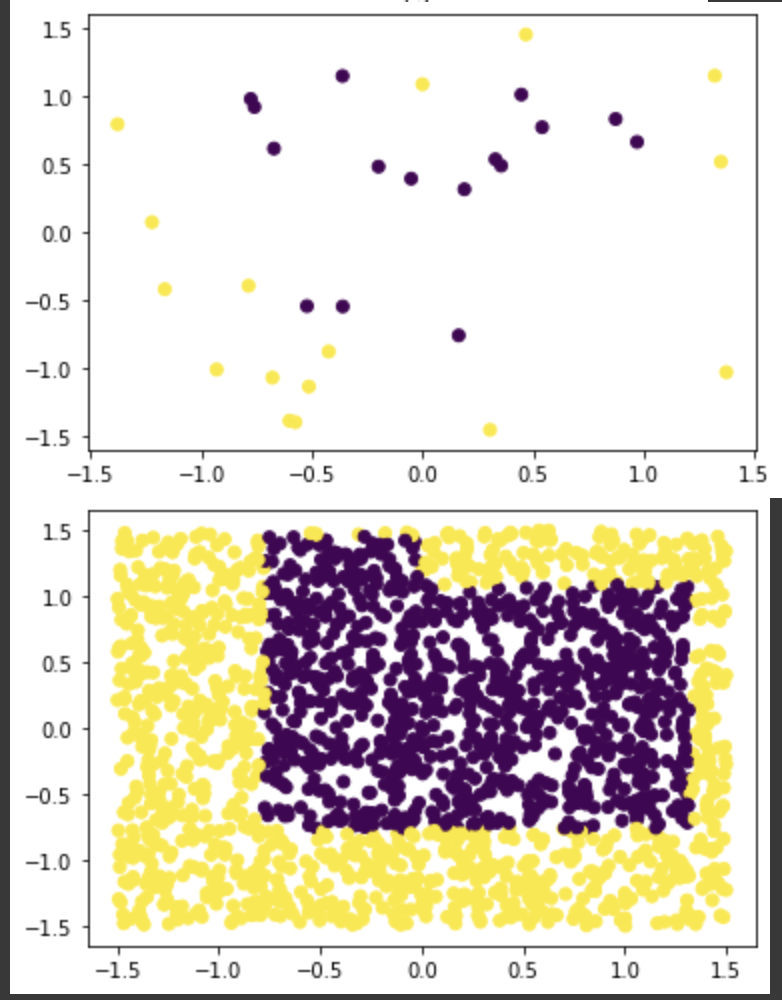
\includegraphics[scale=0.5]{32.png}
            \caption{n=32,Train(Top),Test(Bottom)}
            \label{fig:q2}
        \end{subfigure}
        \begin{subfigure}{0.5\textwidth}
            \centering
            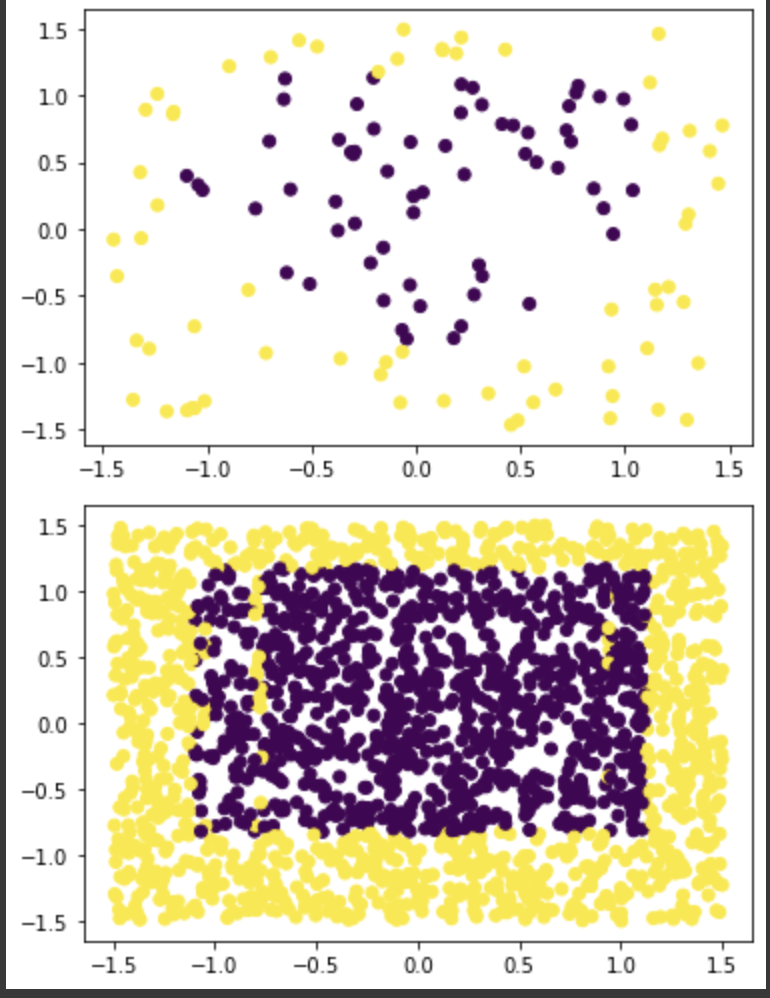
\includegraphics[scale=0.5]{128.png}
            \caption{n=128,Train(Top),Test(Bottom)}
            \label{fig:q2}
        \end{subfigure}
        \end{figure} 
        \begin{figure}[H]
        \begin{subfigure}{0.5\textwidth}
            \centering
            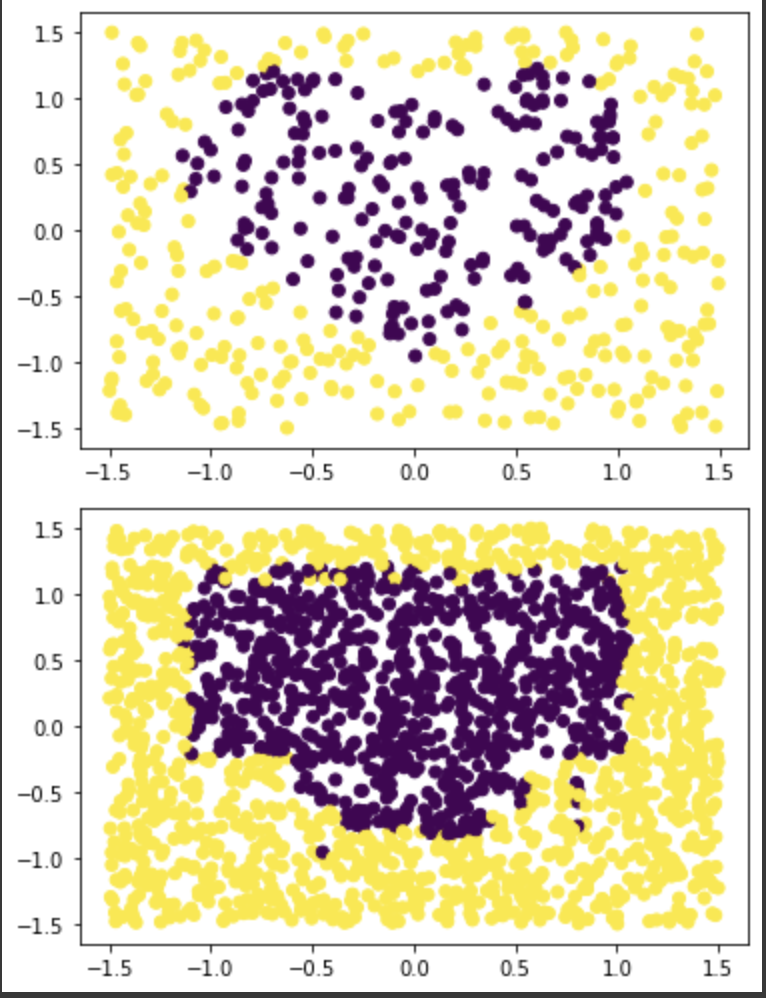
\includegraphics[scale=0.5]{512.png}
            \caption{n=512,Train(Top),Test(Bottom)}
            \label{fig:q2}
        \end{subfigure}
        \begin{subfigure}{0.5\textwidth}
            \centering
            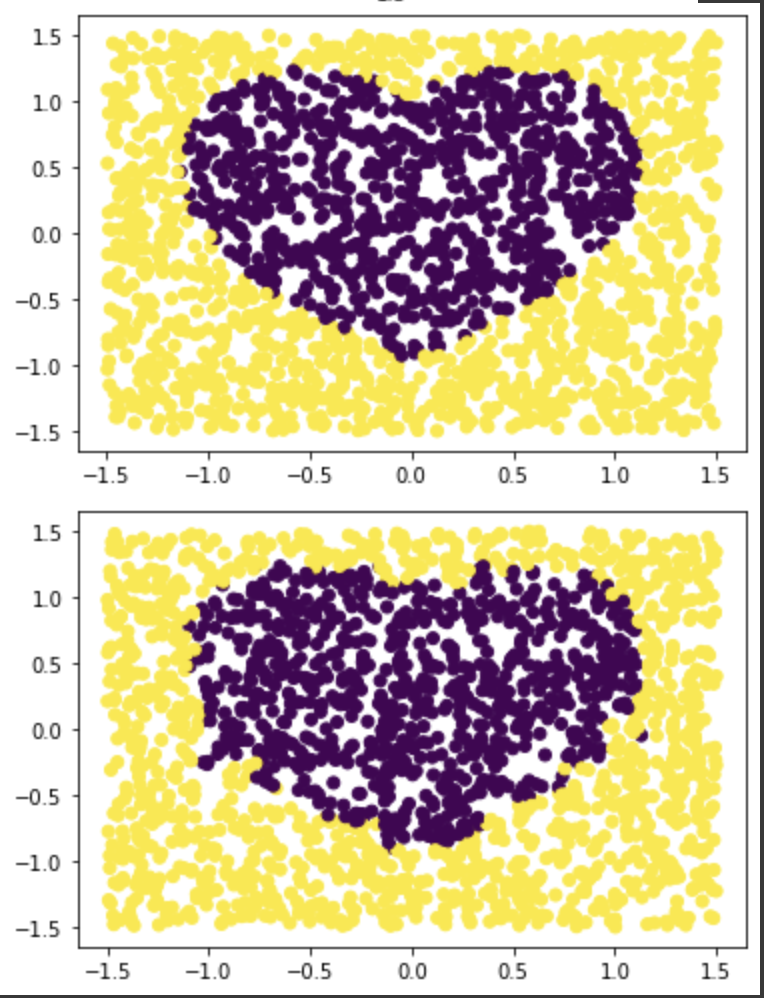
\includegraphics[scale=0.5]{2048.png}
            \caption{n=2048,Train(Top),Test(Bottom)}
            \label{fig:q2}
        \end{subfigure}
        \end{figure} 
        \begin{figure}[H]
            \centering
            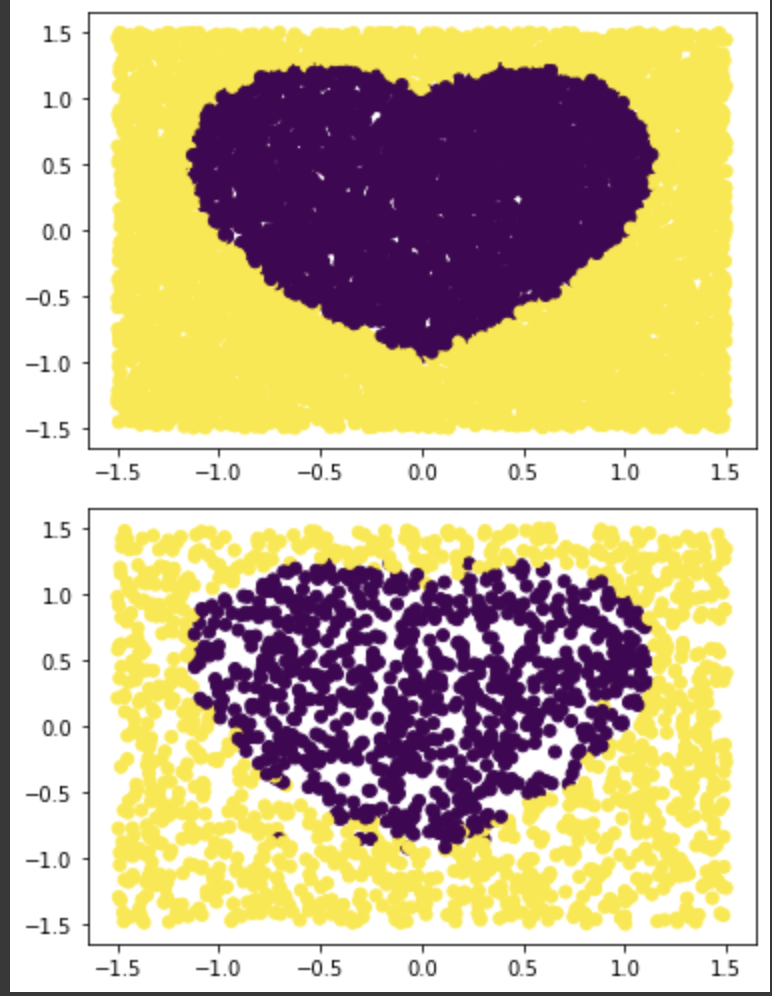
\includegraphics[scale=0.5]{8192.png}
            \caption{n=8192,Train(Top),Test(Bottom)}
            \label{fig:q2}
        \end{figure} 
  \end{soln}
  
\end{enumerate}

\section{sklearn [10 pts]}
Learn to use sklearn (\url{https://scikit-learn.org/stable/}).
Use sklearn.tree.DecisionTreeClassifier to produce trees for datasets $D_{32}, D_{128}, D_{512}, D_{2048}, D_{8192}$.  Show two things in your answer: (1) List $n$, number of nodes in that tree, $err_n$. (2) Plot $n$ vs. $err_n$.\\
\begin{soln}
\begin{center}
    

  \begin{tabular}{|c|c|}
            \hline
            Data Size & Node \\
            \hline
            32 & 11\\
            128 & 19\\
            512 & 53\\
            2048 & 129 \\
            8192 & 249 \\
            \hline
        \end{tabular}\\
  
      Data 32 Split Test Error: 13.38\%\\
      Data 128 Split Test Error: 10.12\%\\
      Data 512 Split Test Error: 4.09\%\\
      Data 2048 Split Test Error: 2.1\%\\
      Data 8192 Split Test Error: 1.0\%\\
      \end{center}
      We can observe the figure below
        \begin{figure}[H]
            \centering
            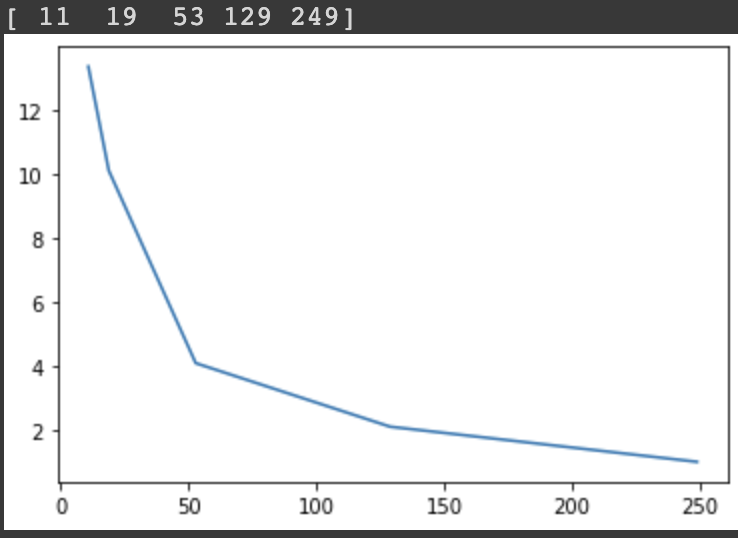
\includegraphics[scale=0.5]{sktest.png}
            \label{fig:q2}
            \caption{Error vs N}
        \end{figure} 
    
    The observed Training and Test plot for 5 splits are shown below:\\
    \begin{figure}[H]
        \begin{subfigure}{0.5\textwidth}
            \centering
            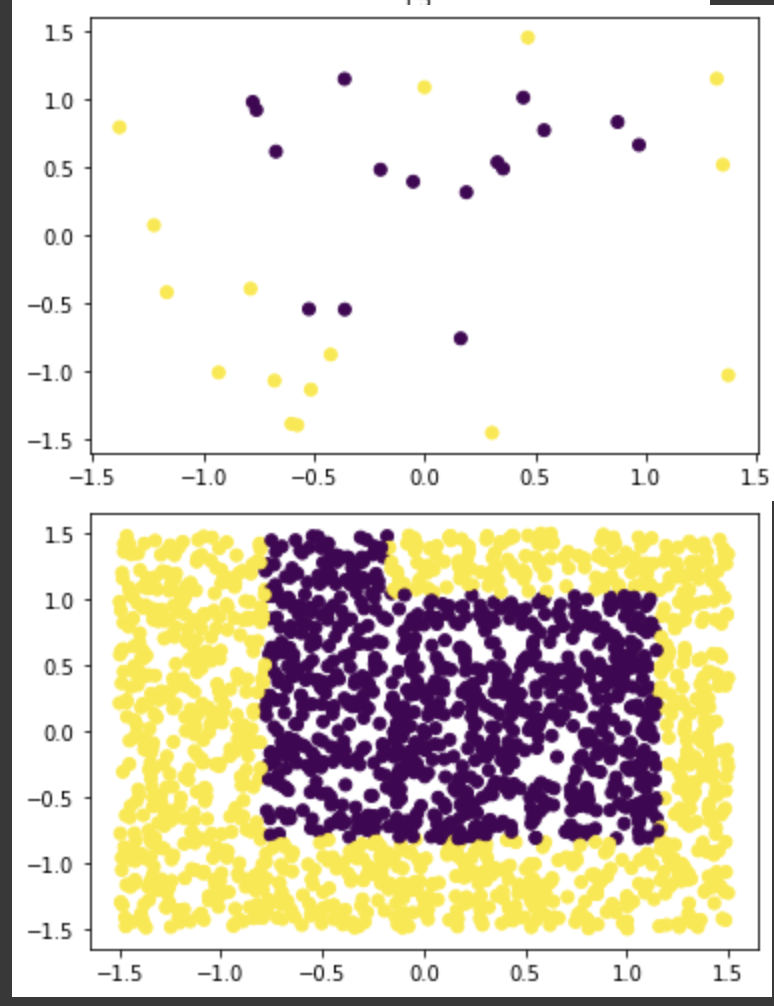
\includegraphics[scale=0.5]{sk32.png}
            \label{fig:q2}
            \caption{n=32,Train(Top),Test(Bottom)}
        \end{subfigure}%
        \begin{subfigure}{0.5\textwidth}
         \centering
            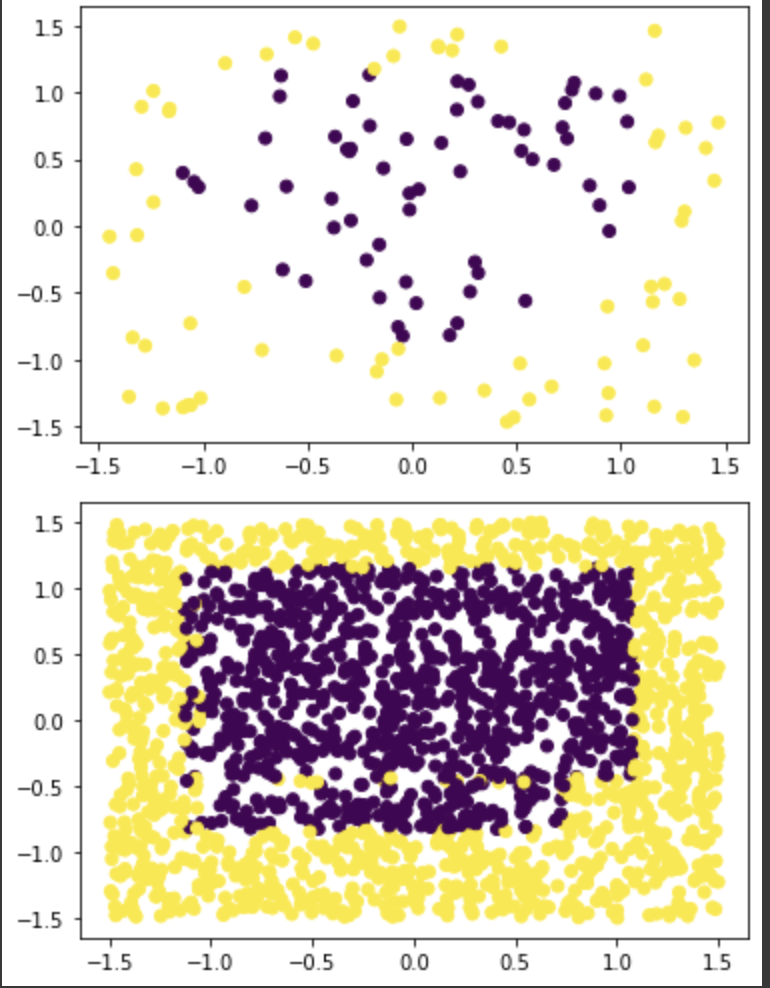
\includegraphics[scale=0.5]{sk128.png}
            \caption{n=128,Train(Top),Test(Bottom)}
            \label{fig:q2}
        \end{subfigure}%
        \end{figure} 
        \begin{figure}[H]
        \begin{subfigure}{0.5\textwidth}
            \centering
            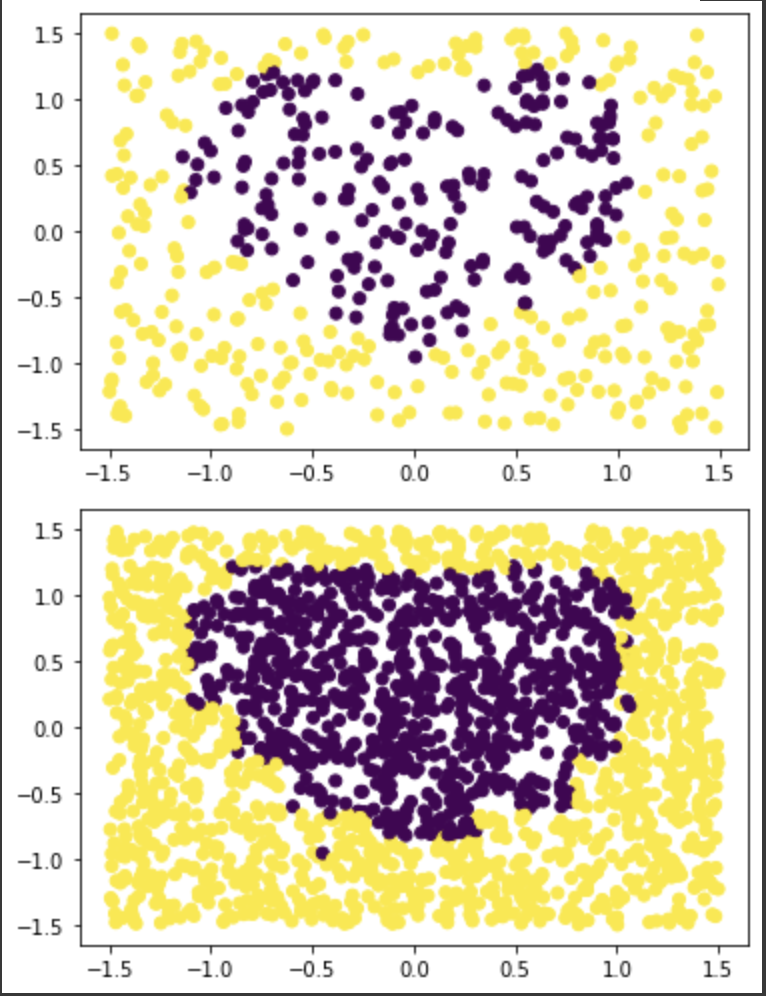
\includegraphics[scale=0.5]{sk512.png}
            \caption{n=512,Train(Top),Test(Bottom)}
            \label{fig:q2}
        \end{subfigure}
        \begin{subfigure}{0.5\textwidth}
            \centering
            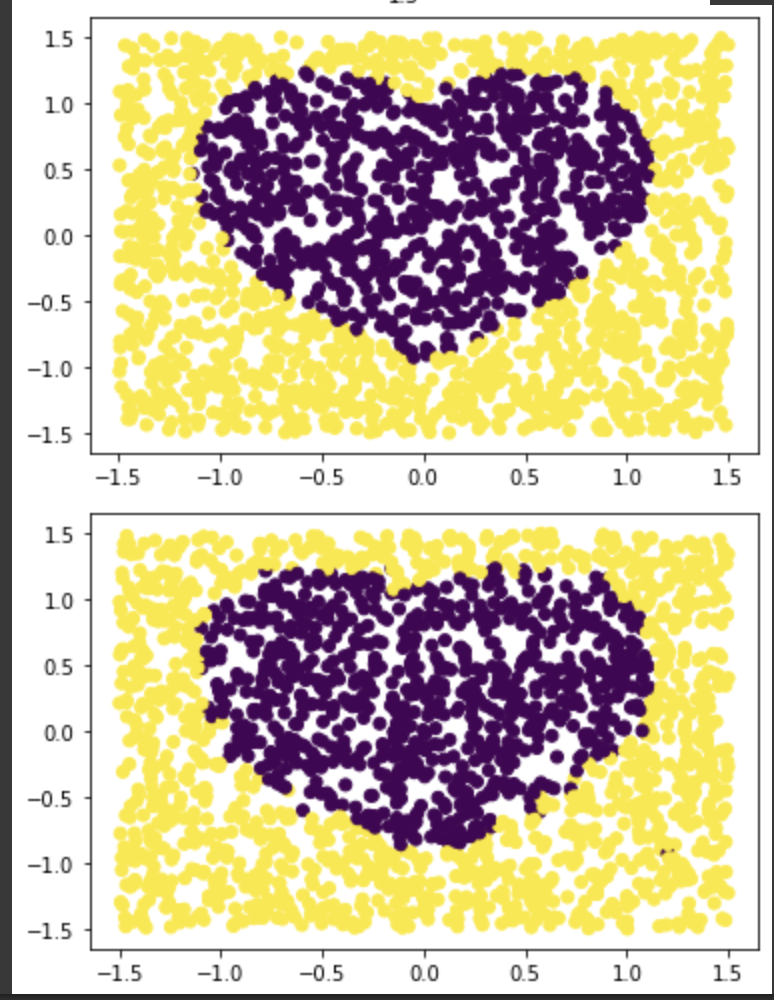
\includegraphics[scale=0.5]{sk2048.png}
            \caption{n=2048,Train(Top),Test(Bottom)}
            \label{fig:q2}
        \end{subfigure}
        \end{figure} 
        \begin{figure}[H]
            \centering
            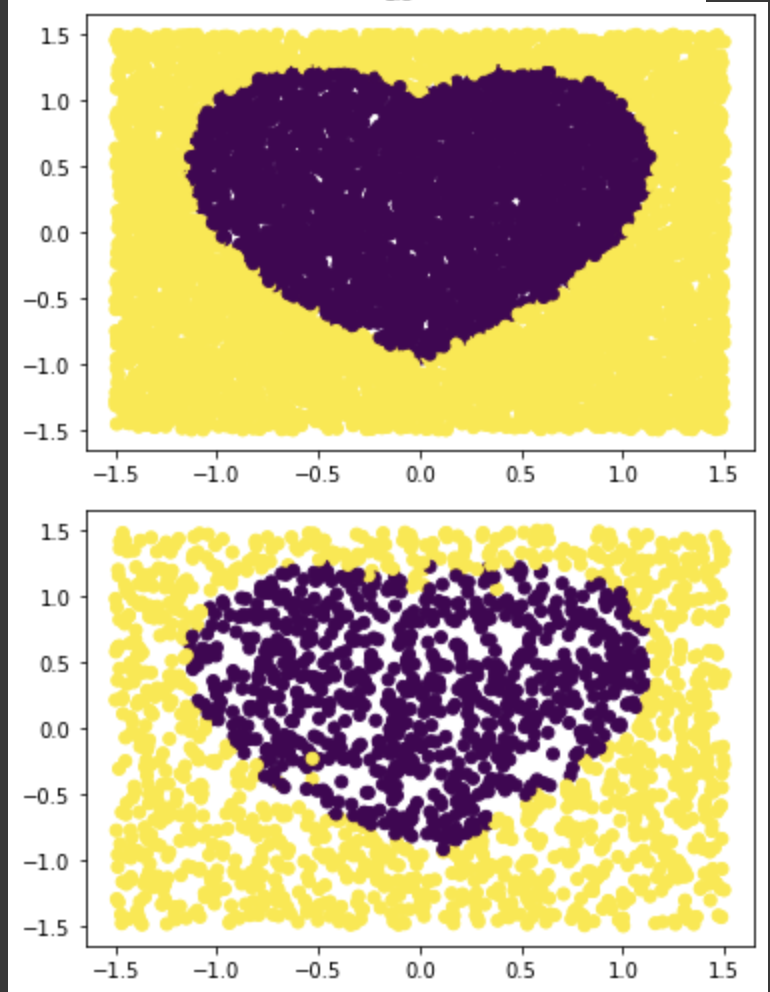
\includegraphics[scale=0.5]{sk8192.png}
            \caption{n=8192,Train(Top),Test(Bottom)}
            \label{fig:q2}
        \end{figure} 
  \end{soln}
  
\section{Lagrange Interpolation [10 pts]}
Fix some interval $[a, b]$ and sample $n = 100$ points $x$ from this interval uniformly. Use these to build a training set consisting of $n$ pairs $(x, y)$ by setting function $y = sin(x)$. \\

Build a model $f$ by using Lagrange interpolation, check more details in \url{https://en.wikipedia.org/wiki/Lagrange_polynomial} and \url{https://docs.scipy.org/doc/scipy/reference/generated/scipy.interpolate.lagrange.html}. \\

Generate a test set using the same distribution as your test set. Compute and report the resulting model’s train and test error. What do you observe?
Repeat the experiment with zero-mean Gaussian noise $\epsilon$ added to $x$. Vary the standard deviation for $\epsilon$ and report your findings.\\
\begin{soln}
    We chose $[0,2pi]$ and uniformly sample random points. We then used Scipy Lagranges function.
    Comparing the outputs and MSE for training data and test data we observe the MSE is almost comparable. Also training on 16 sample and 100 samples  show huge margin in MSE.This could be as per the definition of scipy lagrange's as it cannot sample more than 20 points \\
\begin{center}
    

    \begin{tabular}{|c|c|c|}
            \hline
            Sample & Fitting & MSE \\
            \hline
            16 & Training data & 4.464847788851607e-04\\
            100 & Training data  & 9.787942860736771e+67\\
            16 & Test data & 0.00010328874652770993\\
            100 & Test data & 2.0214972504395186e+75 \\
            \hline
        \end{tabular}\\
        \end{center}
    \begin{figure}[H]
    \begin{subfigure}{0.5\textwidth}
            \centering
            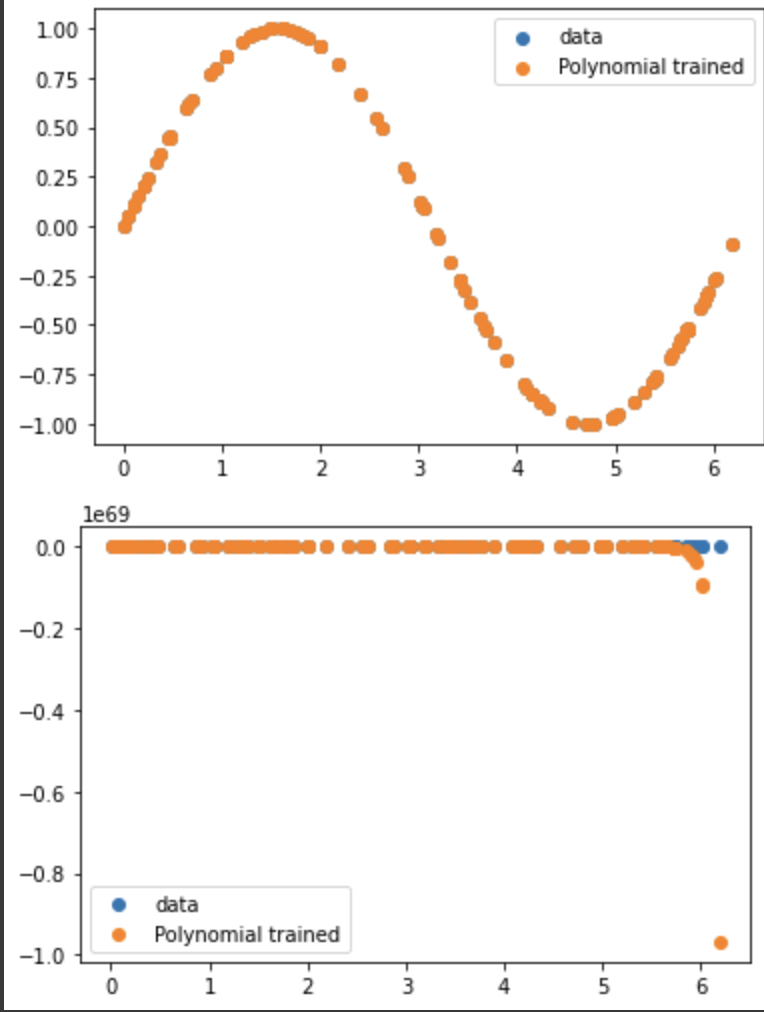
\includegraphics[scale=0.5]{train.png}
            \caption{Fitting on Training test,16 point(Top),100 point(Bottom)}
            \label{fig:q2}
            \end{subfigure}%
             \begin{subfigure}{0.5\textwidth}
            \centering
            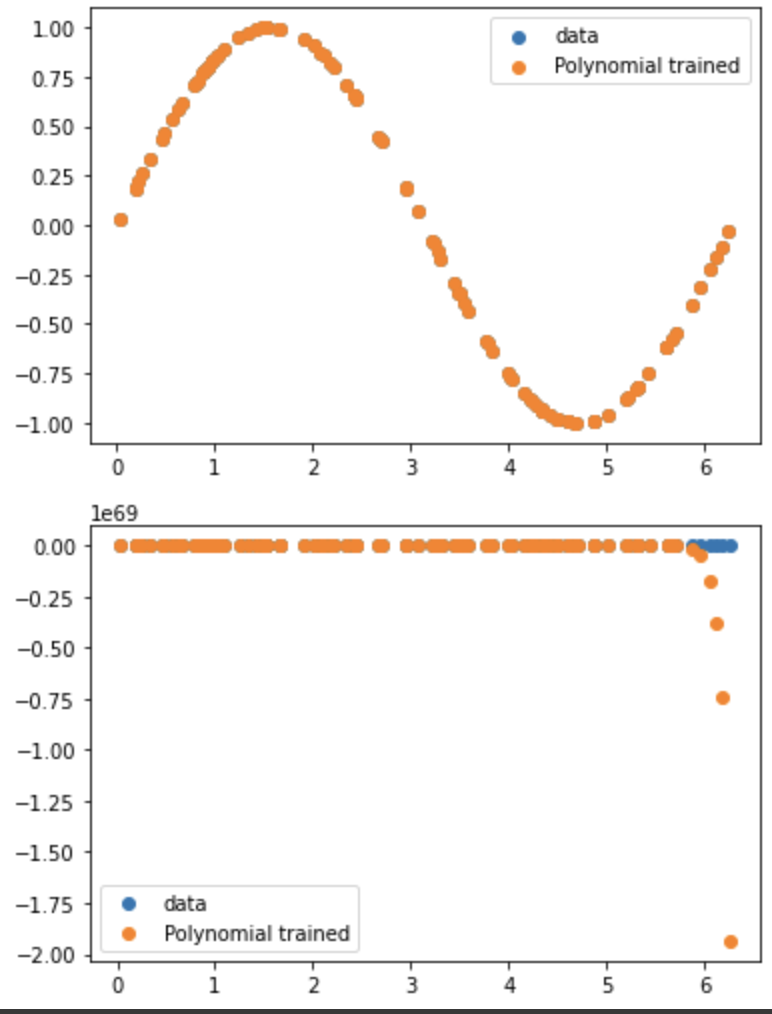
\includegraphics[scale=0.5]{test.png}
            \caption{Fitting on Test set,16 point(Top),100 point(Bottom)}
            \label{fig:q2}
                \end{subfigure}
        \end{figure}
        Adding Gaussian noise we observe that the performance on training data is found to be good but when we pass the Test data in the Lagrange polynomial we find a huge MSE. The plot along with fitting with 16 samples is below:\\
        \begin{figure}[H]
        \begin{subfigure}{0.5\textwidth}
            \centering
            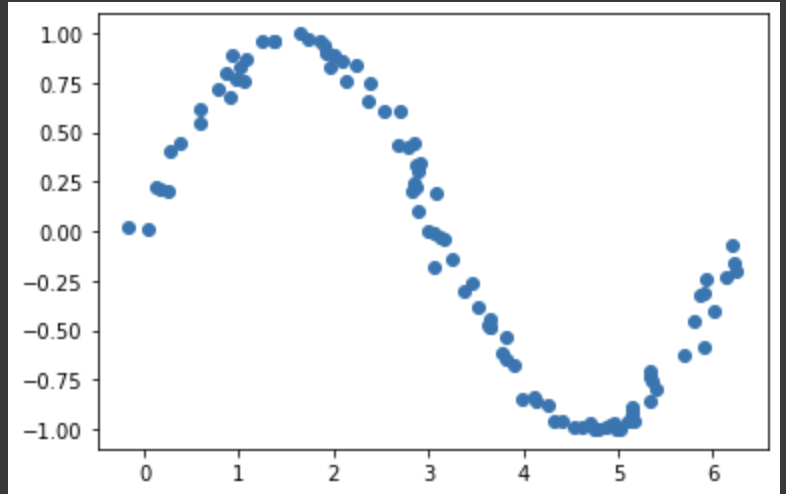
\includegraphics[scale=0.5]{0.1GNoise.png}
            \caption{0 mean 0.1 STD Gaussian Noise}
            \label{fig:q2}
            \end{subfigure}%
            \begin{subfigure}{0.5\textwidth}
            \centering
            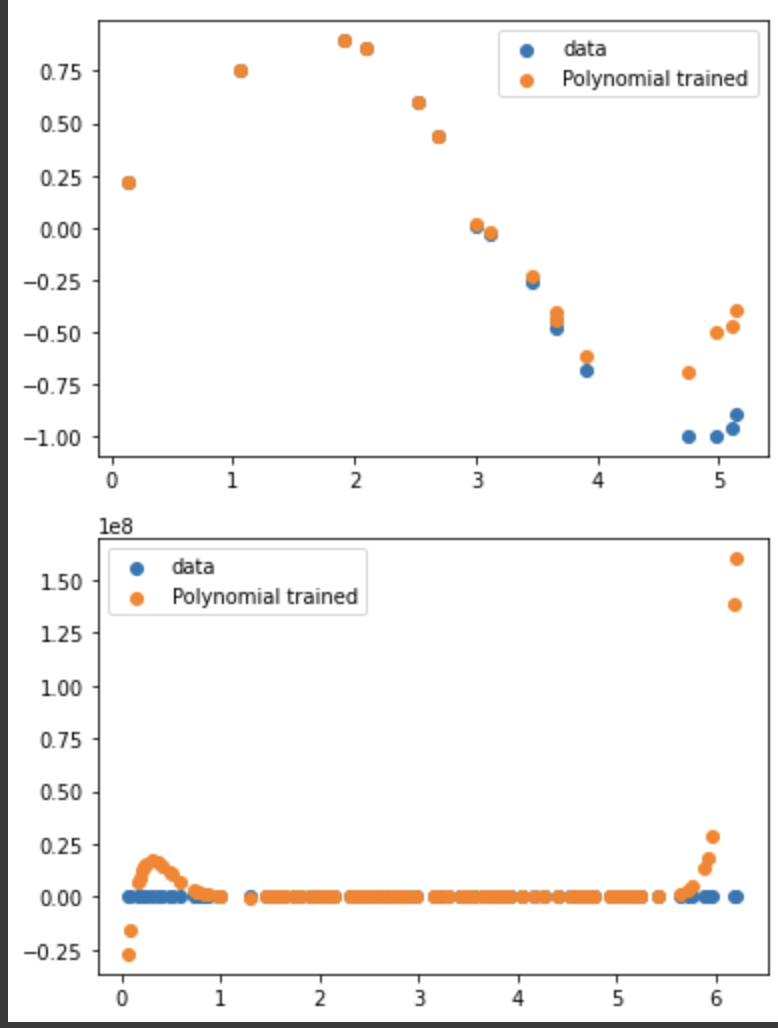
\includegraphics[scale=0.5]{TrnTest.png}
            \caption{Fitting on Training Data(Top),Fitting on Test Data(Bottom)}
            \label{fig:q2}
            \end{subfigure}%
        \end{figure} 
        \begin{center}
            
      
        \begin{tabular}{|c|c|c|}
            \hline
            STD &Data Type & MSE \\
            \hline
            0.01 & Training & 0.0022935\\
            0.01 & Test & 0.18972.49302\\
            0.1 & Training & 0.2282867\\
            0.1 & Test & 22150941.843\\
            0.5 & Training & 0.003901522\\
            0.5 & Test & 12128392.538\\
            2 & Training & 0.0006177\\
            2 & Test & 2585.0242\\
            
            
            \hline
        \end{tabular}\\
          \end{center}
    We observe that as STD increases the MSE on Test Data increases and then decreases. For training data MSE almost maintains itself.
\end{soln}

\bibliographystyle{apalike}
\end{document}
